\documentclass[10pt, a4paper]{article} % Changed to 11 / 10?
\usepackage{geometry}
\usepackage{enumitem} 
\usepackage{titlesec}
\usepackage{booktabs}
\usepackage{tabularx}
% In your preamble:
\usepackage{pdfpages}

% Where you want it in the document:


\geometry{left=2cm, right=2cm, top=2cm, bottom=2cm}
\pagenumbering{gobble}

\titleformat*{\section}{\large\bfseries}
\titleformat*{\subsection}{\normalsize\bfseries}

\date{}
\begin{document}
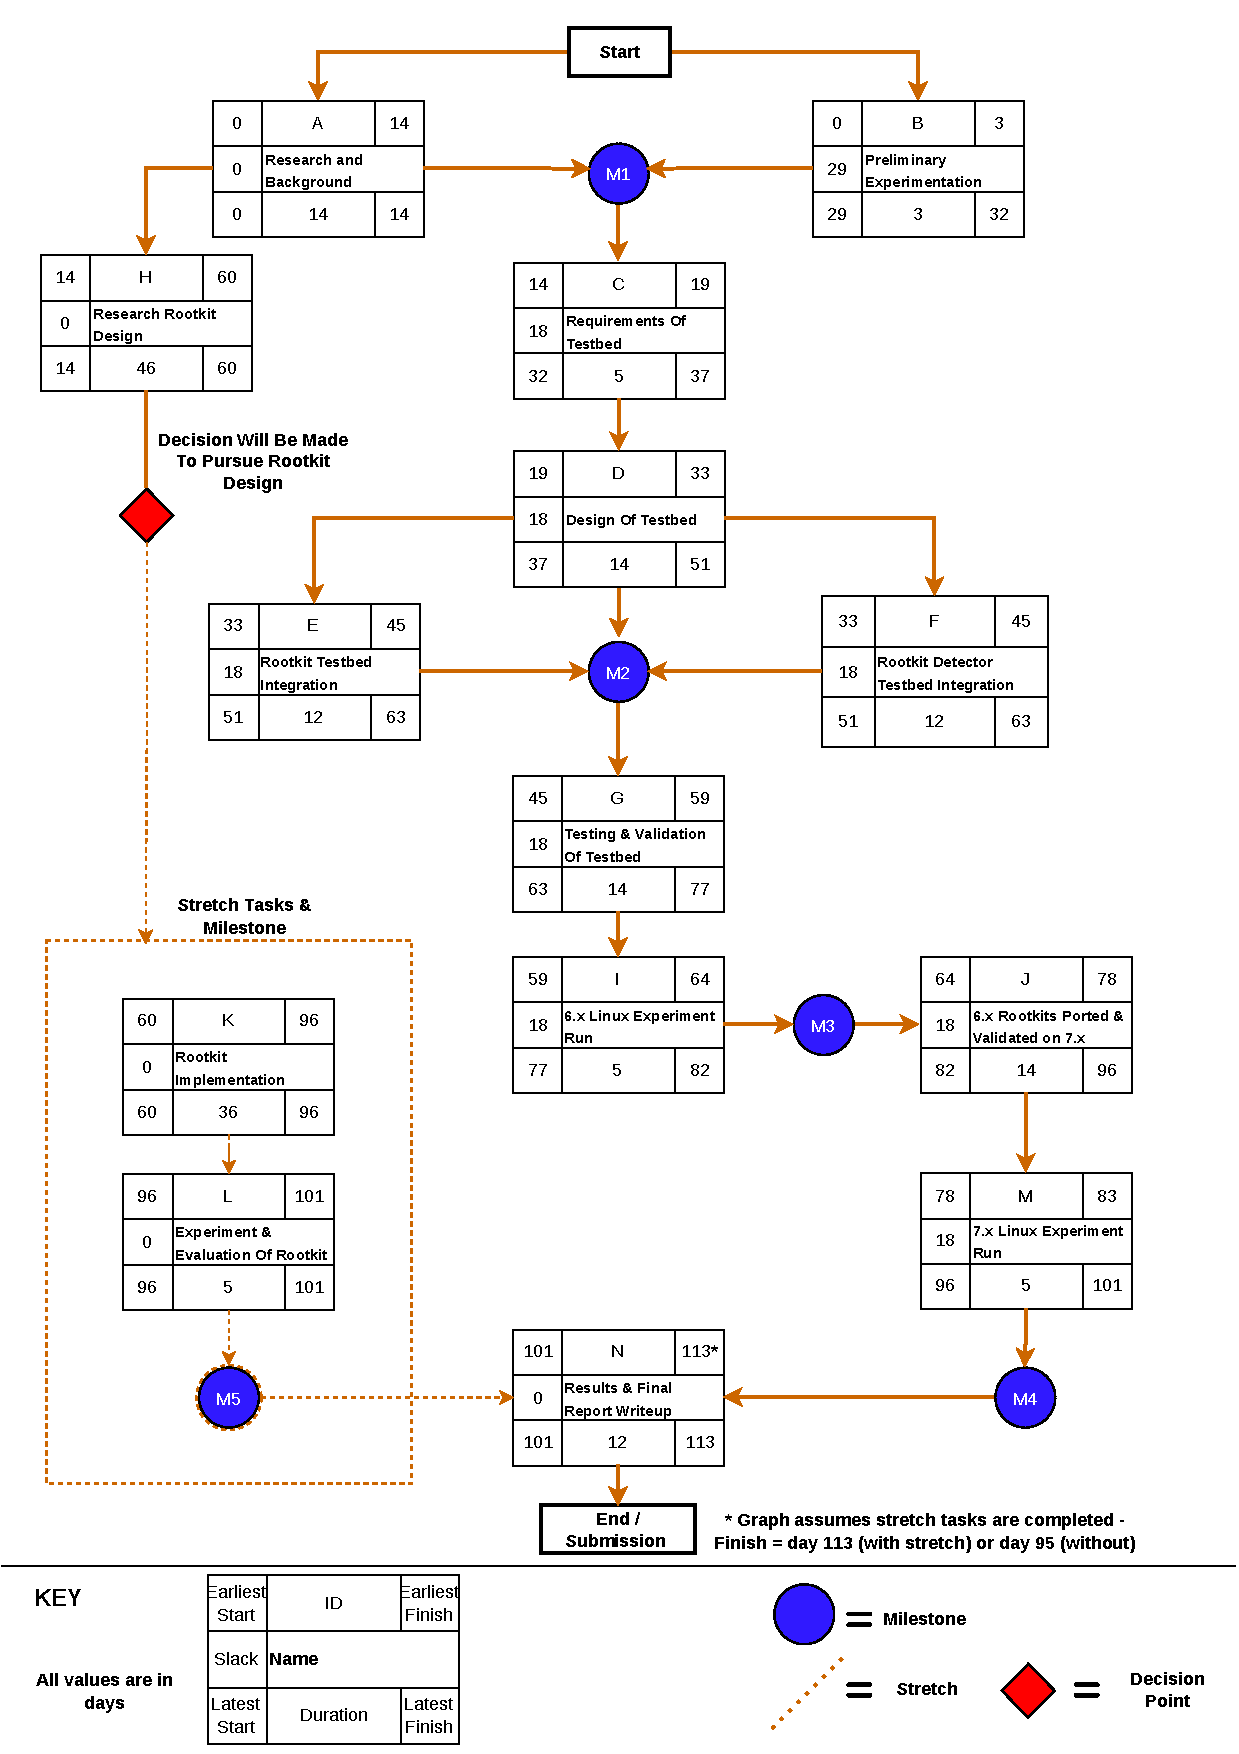
\includepdf[pages=-]{PertDone.pdf}

\noindent{\Large\bfseries ECSP3000 - Plan \& Milestones}\\[10pt]
{\small Elliott Jelbert \quad ej1g24@soton.ac.uk \quad Supervisor: Dr BooJoong Kang}
\vspace{15pt}
% \\ \small Agreed Project Title: A Reproducible Evaluation of Linux Rootkit Detectors via the Implementation of an Automated Testbed \& Proof-of-Concept Rootkit\\[10pt]
\hrule

\section*{Project Plan - PERT \& Gantt Chart}
The PERT chart was used to map out the dependencies of the different tasks \& milestones within my project. The values on the graph use
an expected time - in days - calculated from the optimistic, most likely and pessimistic time estimates.  \\  \\  
The stretch track will be developed in parallel with the rest of the project starting after initial research is complete. A decision will be made after milestone \textbf{M3} (Est. January) as to if a complete rootkit design will be pursued, contigent on time \& feasibility. \\ \\
The PERT Expected Time values were then used to produce a Gantt Chart, mapped against calendar months to help better visualise my project's planned progress against deadlines \& projected milestones.

\subsection*{Tasks}
\begin{table}[h]
  \centering
  \begin{tabular}{|c|l|c|c|c|c|}
    \hline
    \textbf{ID} & \textbf{Task} & \textbf{O} & \textbf{M} & \textbf{P} & \textbf{TE} $= \lceil (O+4M+P)/6 \rceil$ \\
    \hline
    A & Research \& Background       & 7  & 14 & 21 & 14 \\
    \hline
    B & Preliminary Experimentation         & 2  & 3  & 4  & 3  \\
    \hline
    C & Requirements of Testbed       & 3  & 5  & 7  & 5  \\
    \hline
    D & Design of Testbed      & 7  & 14 & 18 & 14 \\
    \hline
    E & Rootkit Testbed Integration           & 7  & 12 & 14 & 12 \\
    \hline
    F & Rootkit Detector Testbed Integration             & 7  & 12 & 14 & 12 \\
    \hline
    G & Testing \& Validation of Testbed & 7 & 14 & 17 & 14 \\
    \hline
    H & Research Phase 2 - Rootkit Design & 30 & 45 & 65 & 46 \\
    \hline
    I & 6.x Linux Experiment Run & 3 & 4 & 7 & 5 \\
    \hline
    J & 6.x Rootkits Ported \& Validated on 7.x & 7 & 14 & 21 & 14 \\
    \hline
    K & Rootkit Implementation & 28 & 36 & 42 & 36 \\
    \hline
    L & Experiment \& Evaluation of Rootkit & 3 & 4 & 7 & 5 \\
    \hline
    M & 7.x Linux Experiment Run & 3 & 4 & 7 & 5 \\
    \hline
    N & Results \& Report Writeup & 7 & 12 & 14 & 12 \\
    \hline
    \multicolumn{5}{|r|}{\textbf{Total}} & \textbf{197} \\
    \hline
  \end{tabular}
\end{table}

\subsection*{Milestones}

These are the milestones I have defined as the major points of progress within my project.
\begin{table}[h]
  \centering
  \begin{tabular}{|c|p{6cm}|p{6cm}|c|}
    \hline
    \textbf{ID} & \textbf{Name} & \textbf{Description} & \textbf{Est. Completed} \\
    \hline
    M1 & Research \& Feasibility Completed  & Finished background research \& completed some initial experimentation. & Early-Nov 2026 \\
    \hline
    M2 & Testbed \& Integration Complete & Testbed design completed \& detectors/rootkits integrated. & Mid-Dec 2026 \\
    \hline
    M3 & 6.x Experiment Data Analysed & Collected \& analysed data from the 6.x experiment run. & Mid-Jan 2027 \\
    \hline
    M4 & 7.x Experiment Data Analysed & Collected \& analysed data from the 7.x experiment run. & Mid-Feb 2027 \\
    \hline
    M5 & Rootkit Designed \& Evaluated \textbf{(Stretch)} & Rootkit has been designed, developed and used to evaluate relevant rootkit detectors using the testbed. & Mid-March 2027 \\
    \hline
  \end{tabular}
\end{table}
\end{document}